\documentclass[compress]{beamer}
\usepackage[utf8]{inputenc}
\usepackage{natbib,amsmath,calc,amssymb,graphicx,tabularx,xr,multirow,times,enumitem,array}
%\usepackage[T1]{fontenc}
%\usepackage{default}
\usepackage{hyperref}
\usetheme{Singapore}
% \usecolortheme{beetle}
\definecolor{anthracite}{RGB}{0,0,0}
\definecolor{grey}{RGB}{150,150,150}
\setbeamercolor{background canvas}{bg=anthracite, fg=white}
\setbeamercolor{background}{fg=white, bg=anthracite}
\setbeamercolor{frametitle}{bg=anthracite,fg=white}
\setbeamercolor{title}{fg=white, bg=anthracite}
\setbeamercolor{normal text}{fg=white,bg=anthracite}

% \setbeamercolor{palette primary}{fg=white, bg=anthracite}
% \setbeamercolor{palette secondary}{fg=white, bg=anthracite}
% \setbeamercolor{palette tertiary}{fg=white, bg=anthracite}
% \setbeamercolor{palette quaternary}{fg=white, bg=anthracite}
\setbeamercolor{local structure}{fg=white, bg=anthracite}
\setbeamercolor{structure}{fg=white, bg=grey}
\setbeamercolor{section in head/foot}{fg=white, bg=anthracite}

\usepackage[T1]{fontenc}


%add the little bullets for the slides
\useoutertheme{miniframes}
\usepackage{etoolbox}
% \usepackage{enumitem}
\usepackage{multimedia}
\makeatletter

%%%%
%%%% THIS MAKES SOME NAVIGATION CYRCLES DISAPPEAR BY USING THE COMMANDS \miniframesoff or \miniframeson : useful for skipping title slide or when 
%there are too many slides
%%%%
\useoutertheme[subsection=false]{miniframes}
\let\beamer@writeslidentry@miniframeson=\beamer@writeslidentry
\def\beamer@writeslidentry@miniframesoff{%
  \expandafter\beamer@ifempty\expandafter{\beamer@framestartpage}{}% does not happen normally
  {%else
    % removed \addtocontents commands
    \clearpage\beamer@notesactions%
  }
}
\newcommand*{\miniframeson}{\let\beamer@writeslidentry=\beamer@writeslidentry@miniframeson}
\newcommand*{\miniframesoff}{\let\beamer@writeslidentry=\beamer@writeslidentry@miniframesoff}
%%%
%%%

%% essential for showing the bullets!!
\usepackage{remreset}
\@removefromreset{subsection}{section}
\setcounter{subsection}{1}
%%

\setbeamertemplate{navigation symbols}{}

\makeatother


\begin{document}
 
\section{Discussion of exercises 1}
\begin{frame}
\frametitle{Important CPM parameters}
\begin{itemize}
 \item temperature \movie[width=2cm, height=2cm, poster, loop]{}{toohot.mp4} ~~~~~~~~~~  J values %when negative, influence on fluctuations 
 \item ~
 \item $\lambda$ ~~  \movie[width=2cm, height=2cm, poster, loop]{}{solid.mp4}  ~~~~targetvolume: too small vs too large %anisotropy vs computational cost
\end{itemize}
\leavevmode
\\~\\
Guideline: multiplying $J$, $\lambda$ and $T$ by the same constant keeps the dynamics the same 
$T$ and $J$ in order 10, $\lambda$ in order one typically yields decent dynamics.\\
\end{frame}

\begin{frame}
\frametitle{Objections and limitations}
\begin{itemize}
 \item volume fluctuations are required for dynamics %can be used to model static objects
 \item no explicit membrane
 \item When J is lower: more adhesion, more fluctuations
 \item no explicit time scale
 \item computational costs
 \item Do due diligence
\end{itemize}

\end{frame}


\begin{frame}
\frametitle{``minimal'' energy configurations}   
Depending on initial conditions and parameters, reaching the minimal energy configuration may take very long.
\begin{center}
\movie[width=6cm, height=6cm, poster, loop]{
\includegraphics[width=0.45\textwidth]{figures/heart.png}}{slide2.2.mp4} \\
\end{center}
we can also use this in our favour
\end{frame}

\begin{frame}[plain]
%\frametitle{Underlying mechanism in brief}   
\begin{center}
 \textbf{Convergent extension}\\
 or\\
 the importance of where you start from
\end{center}
\end{frame}

\section{Application of diff. adhesion}
\begin{frame}
\frametitle{Differential adhesion and convergent extension}  
\begin{center}
 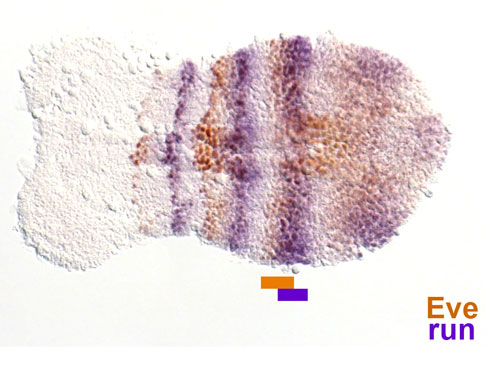
\includegraphics[width=0.6\textwidth]{figures/tribolium_eve_run.jpg}\\
 \tiny from Choe \textit{et al.} 2006
\end{center}

\end{frame}

\begin{frame}
\frametitle{Convergent extension could potentially mess up segments}   
\begin{center}
\movie[width=6cm, height=6cm, poster, loop]{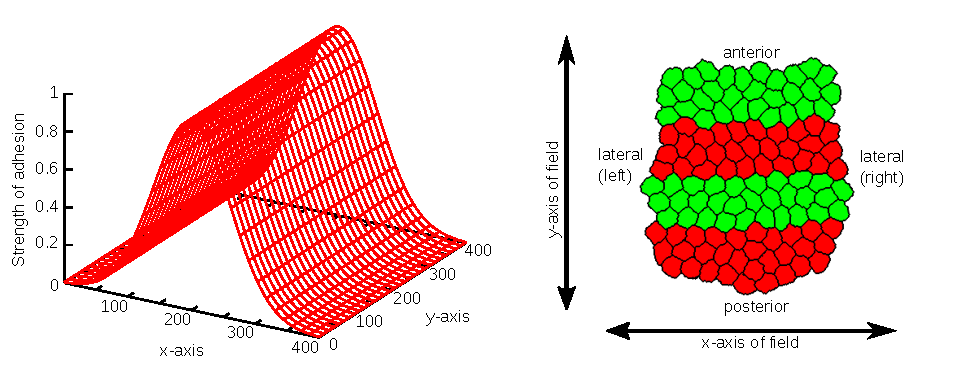
\includegraphics[width=0.7\textwidth]{figures/graded.pdf}}{Video1.mp4} \\
\end{center}
\end{frame}

\begin{frame}
\frametitle{segment-specific adhesion solves this}   
\begin{center}
\movie[width=6cm, height=6cm, poster, loop]{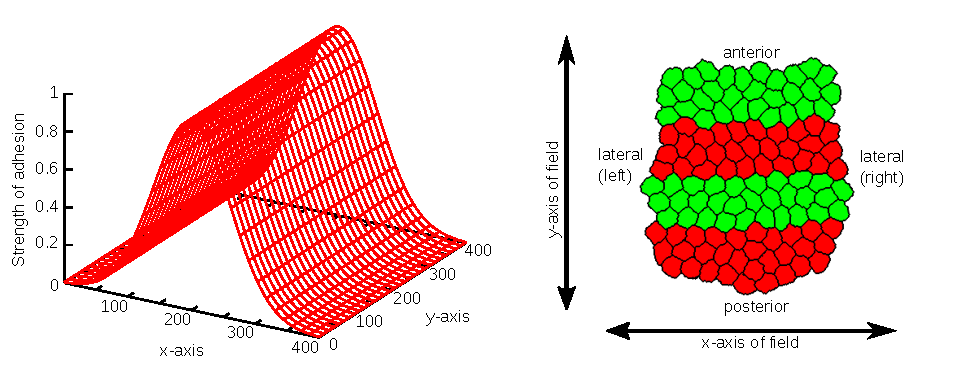
\includegraphics[width=0.7\textwidth]{figures/graded.pdf}}{Video3.mp4} \\
\end{center}
\end{frame}


\begin{frame}
\frametitle{Convergent extension \textbf{by} differential adhesion}   
\movie[width=5cm, height=5cm, poster, loop]{}{Video5.mp4} 
\movie[width=5cm, height=5cm, poster, loop]{}{Video6.mp4} \\
\end{frame}

\begin{frame}
\frametitle{Convergent extension by graded expression of adhesive proteins}   
\begin{center}
 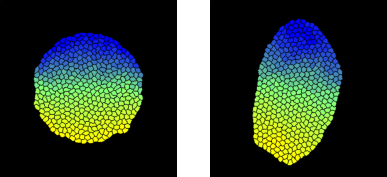
\includegraphics[width=0.9\textwidth]{figures/gradedadhesion.pdf}\\
\end{center}
\end{frame}

\begin{frame}[plain]
%\frametitle{Underlying mechanism in brief}   
\begin{center}
 \textbf{Cell migration}
\end{center}
\end{frame}

\section{Persistent migration}
\begin{frame}
\frametitle{Persistent random walk in T cells}   
% Very \href{https://www.youtube.com/watch?v=g5lhPu24kx4}{\textbf{motile}} cells
\begin{center}
\movie[width=6cm, height=6cm, poster, loop]{}{joost_tcells2p.mpg} \\
\tiny From Beltman \textit{et al}, 2007
\end{center}
``stop-and-go motion''
\end{frame}

\begin{frame}
\frametitle{Underlying mechanism in brief}   
\begin{center}
 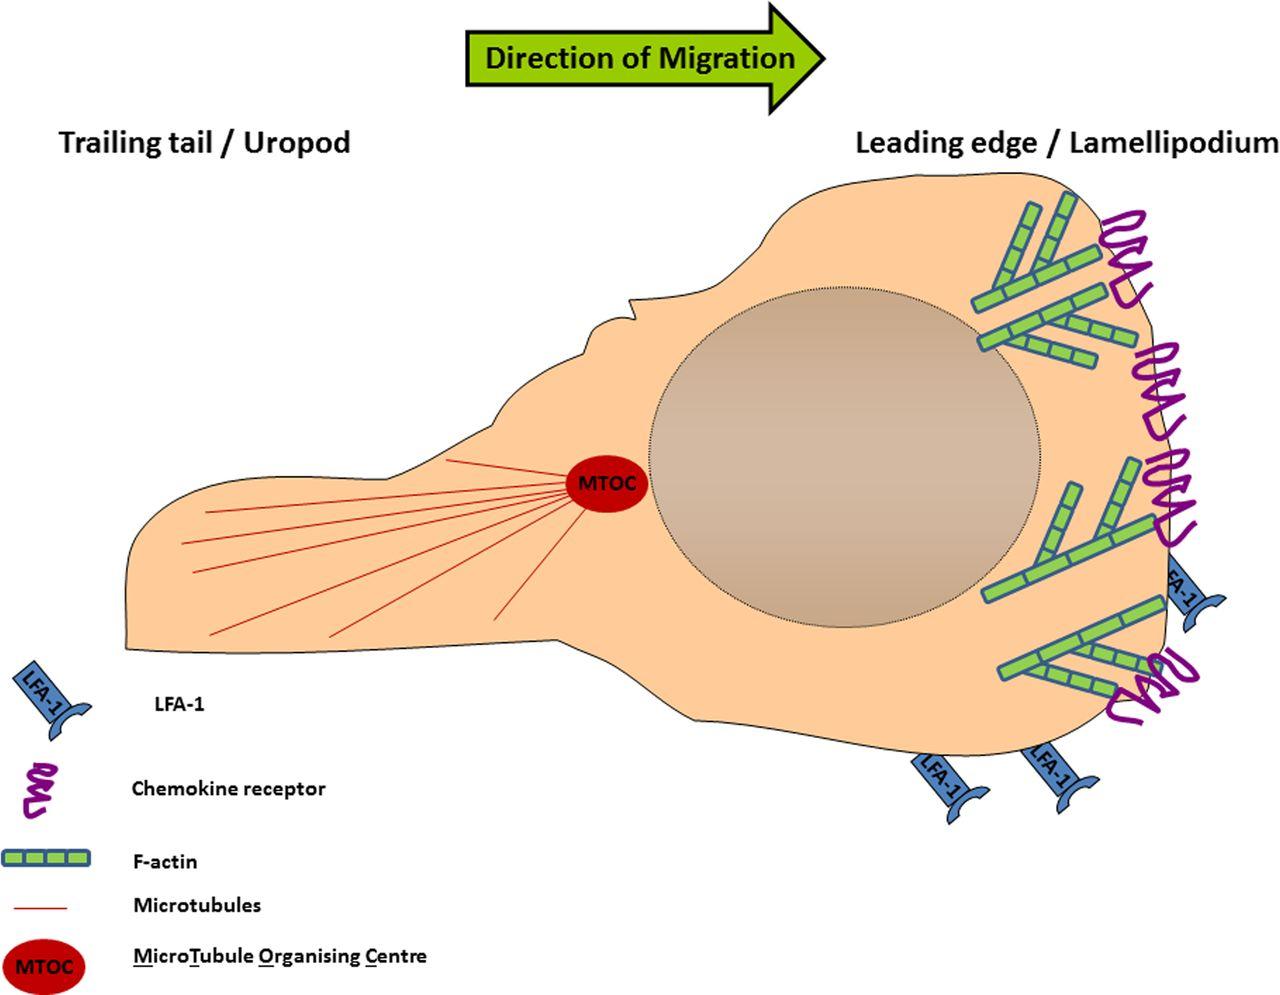
\includegraphics[width=0.9\textwidth]{figures/actinmigration.jpg}\\
\end{center}
\end{frame}

\begin{frame}
\frametitle{Persistent random walk in CPM}   
\[\Delta H += -\mu cos(\alpha)\]
\begin{center}
 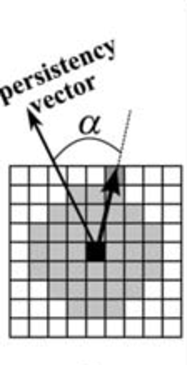
\includegraphics[width=0.2\textwidth]{figures/persistency.pdf}\\
\end{center}
The angle is updated every x timesteps, to reflect the actual direction of motion of the cell\\
~\\
We define this mechanism as change in the Hamiltonian: directly add an extra bias to copy probability 
\end{frame}

\begin{frame}
\frametitle{Exercises part 2}   
\begin{center}
 
\includegraphics[width=0.7\textwidth]{figures/girlnerd.jpg}\\
\end{center}
\end{frame}




% \section{Chemotaxis}
% 
% \begin{frame}
% \frametitle{Common form of directed migration}   
% [video of real cells]
% \end{frame}
% 
% \begin{frame}
% \frametitle{CPM implementation of chemotaxis}   
% 
% Need an extra grid which contains the chemotactant
% \[\Delta H += \mu(\sigma_{source})(C(source)-C(target))\]
%  
%  Where C is the concentration of the morphogen on the secondary grid.
% \end{frame}
% 
% \begin{frame}
% \frametitle{Sorting and chemotaxis}   
% See Kafer and Hogeweg and Maree 2006
% \end{frame}
% 
% \begin{frame}
% \frametitle{Angiogenesis?}   
% Something by Roeland
% \end{frame}





\section{}
\end{document}
